
\subsection{Kompensation Störgröße Fahrzeug}
\label{headtracking_marker_subsec}

Bei einem stationären Fahrzeug genügt es, die Kopforientierung mittels \acs{IMU}-Daten der Brille zu bestimmen.
Die gesuchte Kopforientierung relativ zum Fahrzeug stimmt dabei mit der Kopforientierung bezüglich der Weltkoordinaten überein.
Sobald sich das Fahrzeug jedoch bewegt, wird die Schätzung der Kopforientierung verfälscht.
Fährt das Fahrzeug beispielsweise eine Kurve, so wird die von der IMU gemessene Drehung als Änderung des Yaw-Winkels der Kopforientierung interpretiert, obwohl der Fahrer in Bezug zum Fahrzeug weiterhin geradeaus blickt.

Eine weitere Störquelle stellt die Fahrzeugelektronik und die damit einhergehenden Änderungen des Magnetfelds dar.
Diese Störungen wirken sich negativ auf das zur Driftkorrektur eingesetzte Magnetometer aus (siehe Abschnitt \ref{headtracking_magnetometer_subsubsec}).

Zur Korrektur der Fehlschätzung aufgrund der genannten Einflüsse werden zwei Ansätze untersucht, die die Bestimmung der Kopforientierung relativ zum Fahrzeug stützen.

\begin{figure}[h]
  \centering
  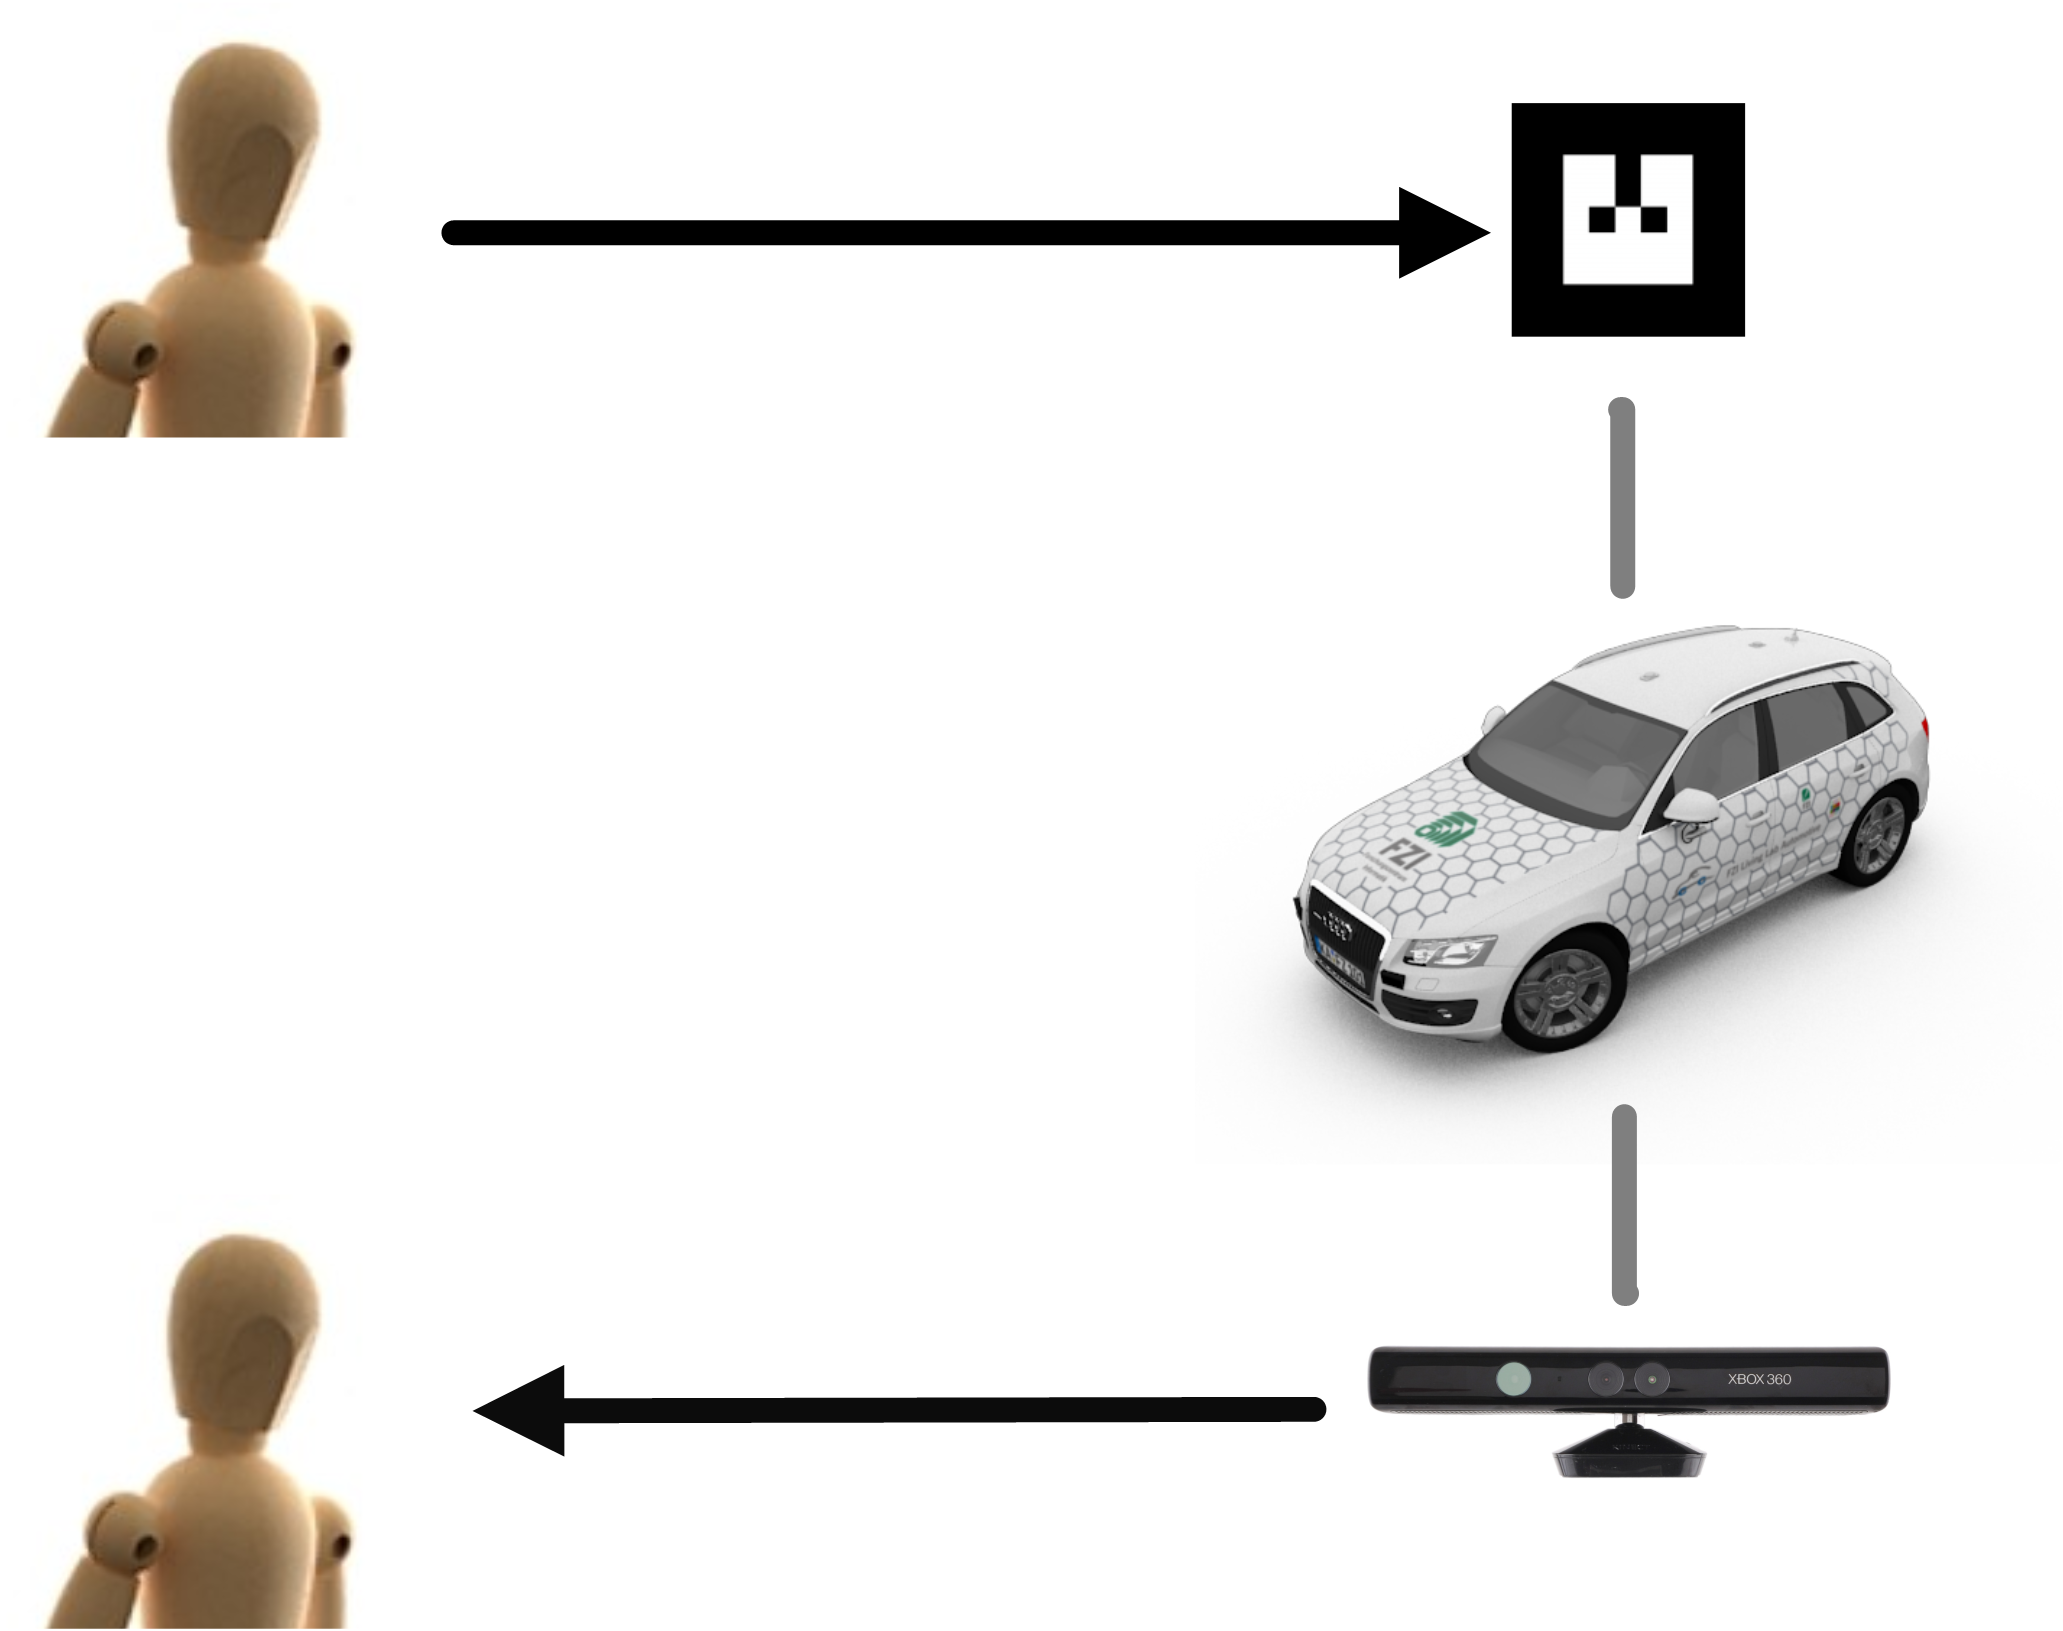
\includegraphics[width=0.4\textwidth]{Tracking_Ansaetze}
  \caption{Tracking-Ansätze: oben: stationärer Marker, bewegliche Kamera; unten: stationäre Kamera, bewegter Kopf}
  \label{fig:tracking_ansaetze}
\end{figure}


\subsubsection{Ansatz: Face-Tracking}

Die Idee beim Face-Tracking-Ansatz ist es, zu untersuchen, inwieweit die bestehende Hardware- und Software-Umgebung des CoCars für die Bestimmung der Kopforientierung verwendet werden kann.
Das Fahrzeug verfügt über eine fest installierte Kinect-Kamera, die auf den Fahrer ausgerichtet ist.
Für diese Kamera wurde am \ac{FZI} bereits ein Algorithmus zur Blickrichtungserkennung des Fahrers implementiert.
Der Algorithmus benutzt dafür ein Gesichtsmodell.
Das Gesichtsmodell berücksichtigt jedoch keine Brille.
Trägt der Fahrer eine Durchsichtbrille, ist ein Teil des Gesichts verdeckt.
Hierdurch wird die Erkennungsleistung stark beeinträchtigt.
Ein möglicher Ausweg ist das Einlernen des Gesichtsmodells mit Brille.
Jedoch ist die Spiegelung der von der Kinect verwendeten Infrarot-Strahlung an der Brille weiterhin problematisch.
Der Ansatz wird aus einem weiteren Grund nicht weiter verfolgt:
Die Verwendung von zusätzlicher Hardware schränkt die Wiederverwendbarkeit des Algorithmus zur Bestimmung der Kopforientierung ein.
Stattdessen fällt die Entscheidung auf einen Marker-Tracking-Ansatz, der alleine mit der Brillen-Hardware auskommt.


\subsubsection{Ansatz: Marker-Tracking}

Beim markerbasierten Tracking handelt es sich um ein optisches Trackingverfahren.
Dabei wird die Position und Orientierung von speziellen Markern bestimmt, die im Kamerabild zu sehen sind.

Verwendung von ALVAR zur Marker-Erkennung

Marker-Kalibrierung (fest im Auto: car -> marker)
Schätzung anhand 3D-Modell (dynamic reconfigure der Marker-Pose)
Schätzung anhand Marker-Pose ermittelt durch ALVAR
Manuelle Ausmessung im realen Fahrzeug

Berechnung der Kopf-Orientierung aus Marker-Orientierung
Inverse
Unterschlagung der position-Information von Alvar

=> Kopf-Orientierung in Auto-Koordinaten



\subsubsection{Fusion IMU und Marker-Tracking}

